\section{Results}\label{results}

\subsection{GPT-5 Benchmarks}

Across the $20$-scenario benchmark, gateway-based architectures achieve substantially higher task effectiveness than the CrewAI baselines on the evaluated models, namely GPT-5, GPT-5-mini, and GPT-5-nano.
With GPT-5 as their backbone, both \emph{Gateway} and \emph{Gateway-RAG} achieve high success scores, indicating that the unified capability gateway yields reliable tasks completion.
The simple pipelines on the other hand perform rather poorly:
\emph{Simple} is excluded from the reported results, as it did not produce meaningful results for comparison.
Reasons are discussed in the following section.
While \emph{Simple-Crew} is able to complete end-to-end pipeline runs, it performs worst across all reported metrics.
The difference in performance compared to the gateway-based architectures is most observable in score, with an absolute gap of nearly $90\%$.
Moreover, while achieving roughly similar input token consumption, the token output of gateway-based architectures is greatly reduced, suggesting less framework-specific verbosity and more efficient agent handoffs.
Finally, \emph{Gateway} outperforms the retrieval-augmented variant across all metrics.

\begin{table}[ht]
\centering
\renewcommand{\arraystretch}{1.2}
\setlength{\tabcolsep}{7pt}

\begin{tabular}{lcccc}
\toprule    & Latency          & Tokens In       & Tokens Out      & Task Score \\
\midrule
Simple      & N/A              & N/A             & N/A             & N/A \\
Simple-Crew & 270.01s          & 67.52k          & 52.24k          & 3.44\% \\
Gateway     & \textbf{188.45s} & \textbf{61.51k} & \textbf{14.21k} & \textbf{93.18\%} \\
Gateway-RAG & 223.04s          & 67.27k          & 15.50k          & 91.09\% \\
\bottomrule
\end{tabular}
\label{fig:gpt-5}

\vspace{4pt}
\par\noindent\normalfont Evaluation Results for GPT-5\par
\end{table}


\subsection{Model Comparison}

Across all tested models, the CrewAI baselines remain ineffective.
Notably, \emph{Simple-Crew}'s quality degrades with increased model capacity:
Starting from $14\%$ task success rate with GPT-5-nano down to $3\%$ with GPT-5, as observable in tables~\ref{fig:gpt-5-nano}, \ref{fig:gpt-5-mini}, and \ref{fig:gpt-5-appendix}.
Also, token consumption increases substantially as models grow larger.

The number of output tokens in both pipelines follows a distinct pattern:
GPT-5-nano consumes the most tokens by far, GPT-5-mini drastically reduces consumption, and with GPT-5 it slightly increases again.

In contrast, \emph{Gateway} scales strongly in task success with model capacity.
Its performance rises from roughly $49\%$ with GPT-5-nano to $89\%$ with GPT-5-mini and above $93\%$ with GPT-5, showing that the architecture already achieves very strong results with the mid-sized model in the compact environment.

\emph{Gateway-RAG} also benefits from increased model capacity, but more gradually and from a much lower starting point.
On GPT-5-nano, the retrieval-augmented variant even underperforms \emph{Simple-Crew} in task success despite being more efficient on the other reported metrics.
With GPT-5-mini and GPT-5, its task success improves substantially, yet it remains below \emph{Gateway} across all tested backbones.
This suggests that retrieval-augmented capability discovery is not beneficial in a perfectly pure environment.

\subsection{Environment Scaling Results}

As already described in subsection~\ref{env-scaling}, starting from the perfectly configured environment, we gradually increase the number of available tools.
Under this growing capability load, both gateway-based variants remain consistent on all reported metrics, with one exception:
\emph{Gateway}'s input token consumption increases roughly proportional to the number of available tools, whereas \emph{Gateway-RAG} remains nearly constant.

\begin{figure}[H]
\centering
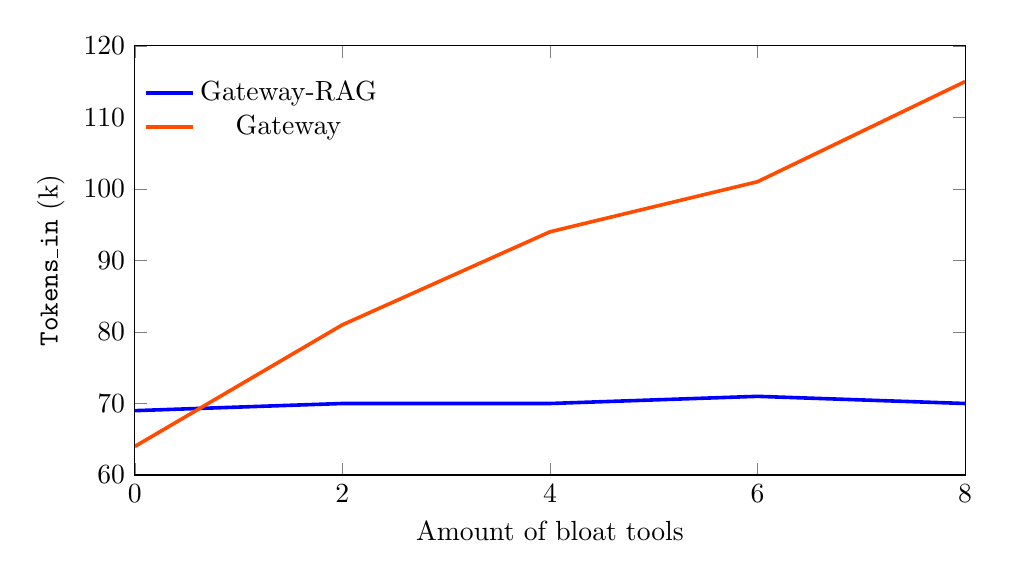
\begin{tikzpicture}
\begin{axis}[
  width=\linewidth,
  height=0.58\linewidth,
  xlabel={Amount of bloat tools},
  ylabel={\texttt{Tokens\_in} (k)},
  xmin=0, xmax=8,
  xtick={0,2,4,6,8},
  ymin=60, ymax=120,
  ytick={60,70,80,90,100,110,120},
  legend style={at={(0,0.85)},anchor=west,draw=none},
]
\addplot[line width=1.3pt,color=blue] coordinates {(0,69) (2,70) (4,70) (6,71) (8,70)};
\addplot[line width=1.3pt,color=red!70!yellow] coordinates {(0,64) (2,81) (4,94) (6,101) (8,115)};
\legend{Gateway-RAG, Gateway}
\end{axis}
\end{tikzpicture}
\caption{\texttt{Tokens\_in} under increasing capability load. Values are in thousands of tokens (k); the y-axis is truncated (60--120k) for readability.}
\label{fig:tokens_in_bloat}
\end{figure}

